To quantify the effectiveness of our method, we compared various metrics manually annotated data, acting as ground truth. 
Further, we also incorporate the same metrics from OpenDataCam.

\subsection{Interpretation of desire paths}
From the trajectory analysis in figure~\ref{Rainbow} we derived eight commonly used desire paths.
We mainly focus on desire lines for south-bound traffic from Skelbækgade (figure \ref{traject}) as referenced in section 4.1.
\ \\

\raggedbottom
\begin{tabular}{@{}cc}
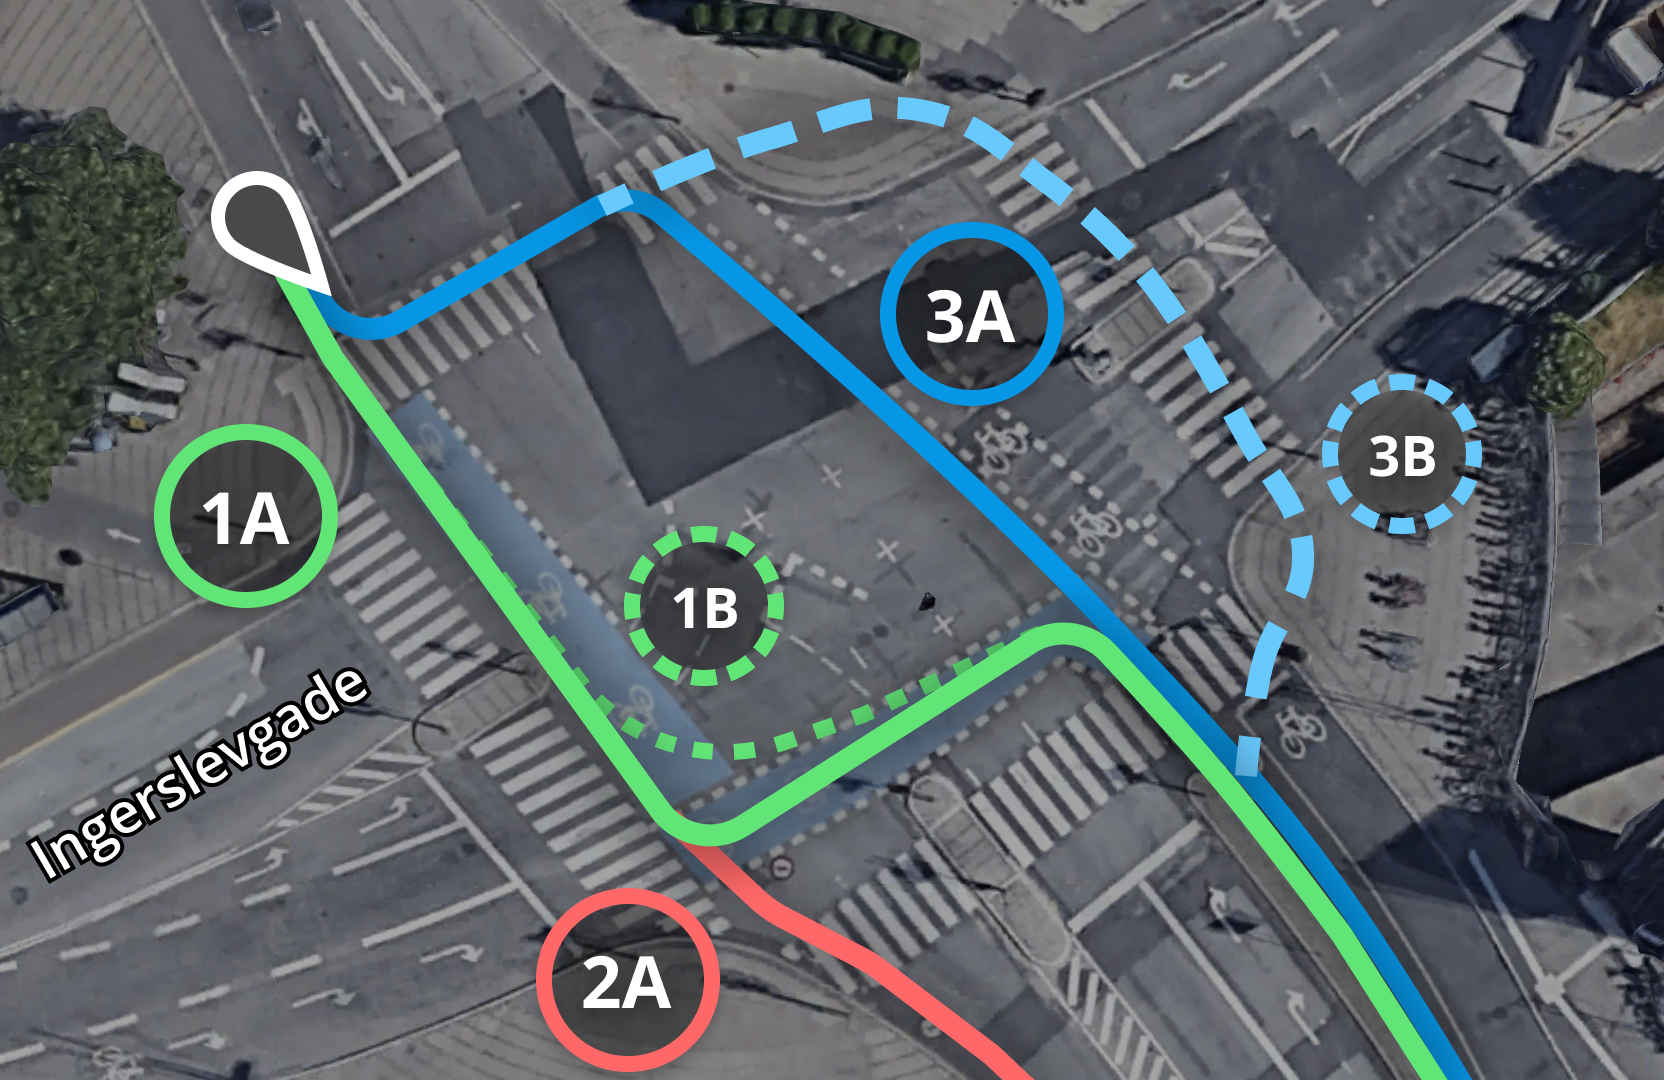
\includegraphics[width=1.0\columnwidth]{desire_paths_overhead} 
\end{tabular}
\captionof{figure}{Common desire lines of cyclists coming from NW}
\label{traject}

\subsection{Desire line counts}
We initiated two uni-directional counting lines in the middle of the intersection as a way to access the traffic volume for desire lines 1 and 3 (fig. \ref{traject}).

In table \ref{tab:comparison_counts} we show a comparison of manually annotated counts, OpenDataCam counting lines, 
and our implementation. The counts are based on 1.5 hours of footage and only counting objects detected as cyclists.

\begin{table}[h]
\resizebox{\columnwidth}{!}{%
\renewcommand{\arraystretch}{2}\begin{tabular}{|c|c|c|c|}
\hline
& \textbf{Manual annotation} & \textbf{Our method}               & \textbf{OpenDataCam}              \\ \hline
\textbf{1 (A+B)} & 192                        & {\color[HTML]{FE0000} 184 (-4\%)} & {\color[HTML]{FE0000} 63 (-67\%)} \\ \hline
\textbf{3 (A+B)} & 99                         & {\color[HTML]{32CB00} 102 (+3\%)} & {\color[HTML]{FE0000} 50 (-49\%)} \\ \hline
\end{tabular}
}
\caption{Comparison of counts}
\label{tab:comparison_counts}
\end{table}

While our counting method got close to the true counts, OpenDataCam captured less than half the cyclists passing its 
counting lines. Further, while the absolute counts of OpenDataCam did not match the manual annotation, 
nor did the proportions between the two counts.
Although the counting line implementation varies between our tool and OpenDataCam, 
the difference can primarily be attributed to the better detection accuracy of bicycles in YOLO5.
\ \\

\subsection{Behavioral analysis}
As mentioned in section 4.3.1, we couple the top-level view with references to timestamps in the recorded footage, 
such that the behavior of cyclists can be observed at street level.
Whenever a unique trajectory is selected, or a part of the intersection is marked off, one can inspect each cyclist 
and the context leading up to a detection.
\\

In figure \ref{Alert1} we see a detection of a cyclist passing straight over Dybbølsbro instead of turning left and 
continuing over the bi-directional cycle path. Unknowingly thinking he is right, he closely passes, at full speed, another rider crossing
the street. Shortly after, he notices the traffic markings and turns around. 

\ \\ 
\raggedbottom
\begin{tabular}{@{}cc}
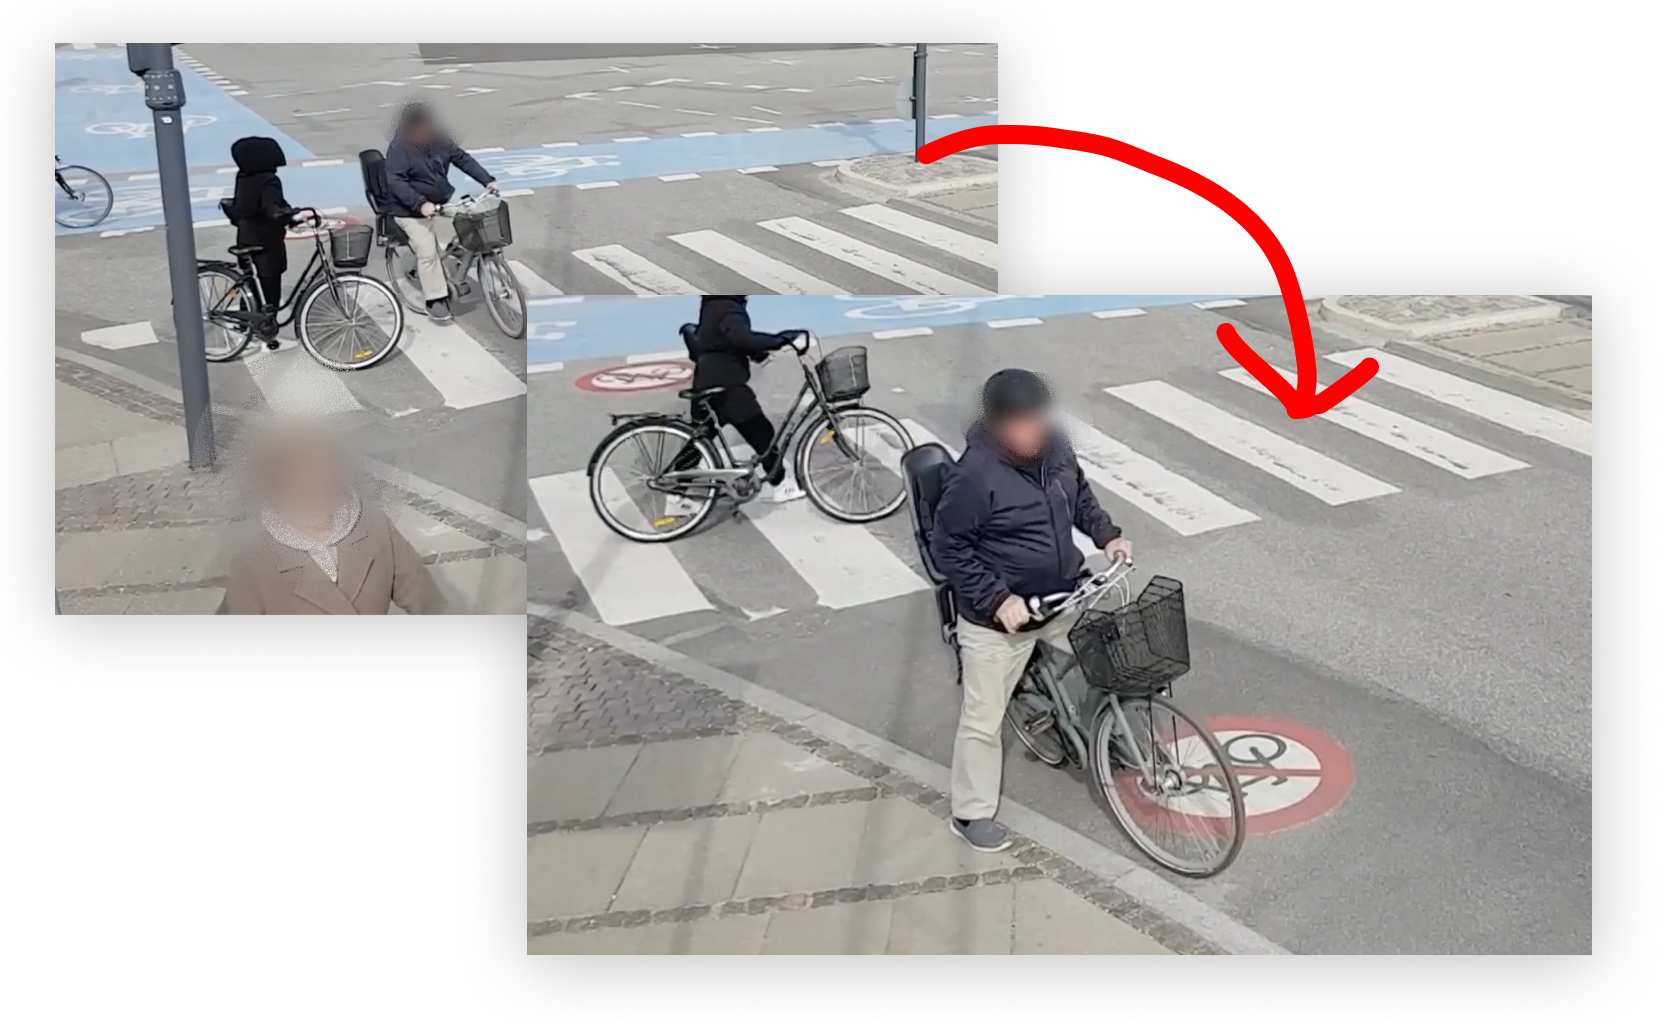
\includegraphics[width=1.0\columnwidth]{behaviour_fast} 
\end{tabular}
\captionof{figure}{Detection zone triggered}
\label{Alert1}
\

Other cyclists (unknowingly) performing the same maneuver all tended to look to their left 
as they passed the pedestrian crossing (examples in appendix A).
As they look, they also steer slightly in the same direction, which can lead to close contact with vehicles
in the narrow car-only lane. 
\ \\

Another commonly observed behavior was cyclists trying to shorten the trajectories of their turns (fig. \ref{Alert2})
at the 'waiting corner' at Ingerslevgade (see desire line \textbf{1B}).

\raggedbottom
\begin{tabular}{@{}cc}
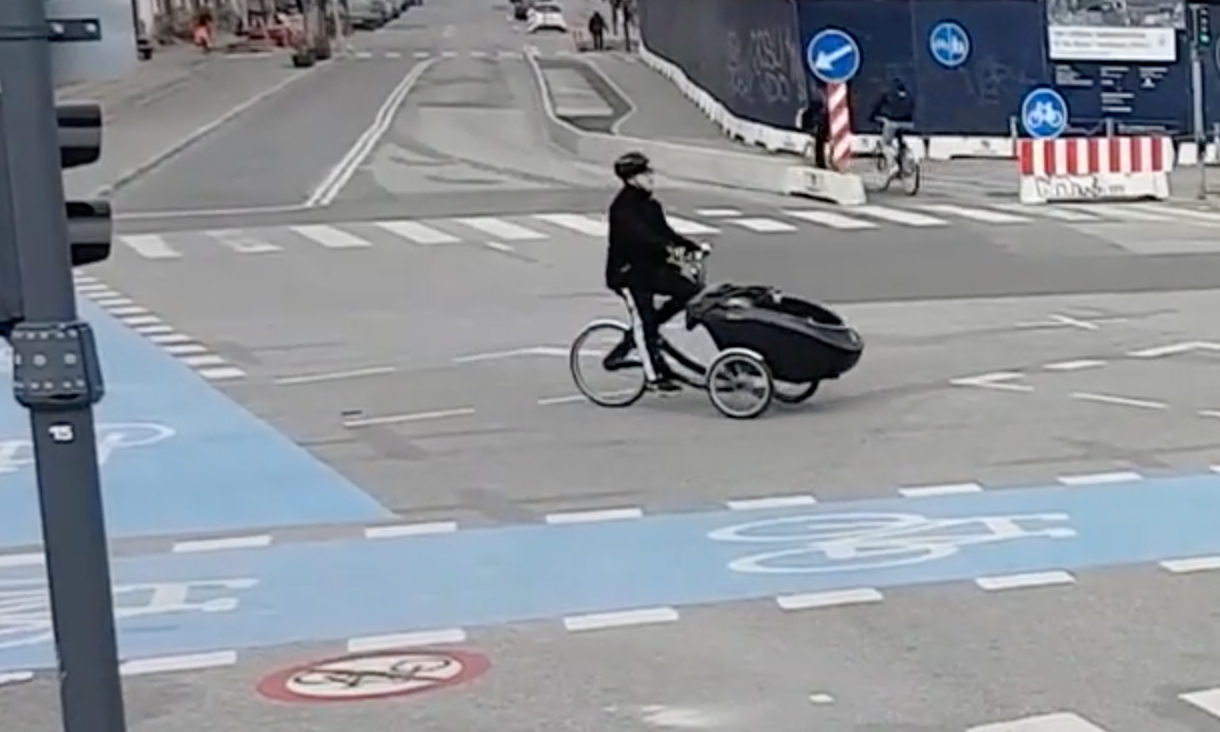
\includegraphics[width=1.0\columnwidth]{shorten_traj} 
\end{tabular}
\captionof{figure}{Shortend left-turn}
\label{Alert2}
\

When volumes of other traffic were low or over the short window of all traffic having red lights, cyclists would use the opportunity 
to swiftly cross the intersection while still 'following the correct path' (that is, not crossing in a fully diagonal path). 

% Which are all compared to the "ground truth" dataset that we annotate manually. We know from previous works with OpenDataCam
% that vehicle detection has achieved 95\% accuracy while performing worse for pedestrians and motorcycles (\cite{BROEKMAN2021100068}).

